% Template for white paper submissions for the 
% LSST Call for Observing Strategies for DeepDrilling and Minisurveys 
% 
% The call for white papers can be found at https://github.com/lsst-pst/survey_strategy/blob/master/latex/WPcall2018.pdf
% The deadline for submissions is November 29, 2018
% Please submit your white paper via a pull request at https://github.com/lsst-pst/survey_strategy_wp, after creating a 
%   subdirectory named LASTNAME_FIRSTNAME_NUMBER
% For help with white papers or the submission process, please post at http://community.lsst.org/c/sci/survey-strategy


\documentclass[11pt]{article}
\usepackage[english]{babel}
\usepackage{amsmath}
\usepackage{amssymb}
\usepackage{graphicx}
\usepackage{hyperref}
\usepackage{wrapfig,verbatim,caption,subcaption,calc,relsize,multicol,enumitem,titlesec}

\usepackage[utf8]{inputenc}
\usepackage{booktabs}
\usepackage[utf8]{inputenc}
\usepackage{natbib}

%Includes "References" in the table of contents
\usepackage[nottoc]{tocbibind}
\def\apj{AstroPhysical Journal}             % Astrophysical Journal
\def\apjl{Astrophysical Journal, Letters}                % Astrophysical Journal, Letters
\def\apjs{Astrophysical Journal, Supplements}               % 

\title{Template for LSST Call For Survey Strategy Optimization White Papers}
\author{}
\date{May 2018}

\begin{document}

\maketitle

\begin{abstract}

Please provide a short summary of your scientific goals and survey strategy modifications here.
\end{abstract}

\section{White Paper Information}
Authors: 

\noindent
\author{Federica B. Bianco, fedhere@gmail.com, CUSP, CCPP, NYU, UDel }

\noindent
\author{Melissa Graham, University of Washington}

\noindent
\author{Maria Drout, Dunlap Institute, University of Toronto}

\noindent
\author{Gautham Narayan, STScI}

\noindent
\author{Igor Andreoni, Caltech}

\noindent
\author{Tyler A Pritchard, NYU} 

\noindent
\author{Tiago Ribeiro, LSST}

\noindent
\author{Philip Cowperthwaite, Carnegie}

\noindent
\author{Rahul Biswas, Stockholm University}

\begin{enumerate} 
\item {\bf Science Category:} Exploring the Transient Sky, Dark Energy
\item {\bf Survey Type Category:} 
The `wide-fast-deep' (WFD) Main Survey. (Although, a Mini-Survey in which only a portion of the sky is observed with our proposed strategy -- or even a Deep Drilling Field --  could be considered.) 
\item {\bf Observing Strategy Category:} 
   a specific observing strategy to enable specific time domain science, that is relatively agnostic to where the telescope is pointed. 
\end{enumerate}  


\clearpage
%%%%%%%%%%%%%%%%%%%%%%%%%%%%%%%%%%%%%%%%%%%%%%%%%%%
\section{Scientific Motivation}
\begin{footnotesize}
{\it Describe the scientific justification for this white paper in the context of your field, as well as the importance to the general program of astronomy, including the relevance over the next decade. Describe other relevant data, and justify why LSST is the best facility for these observations. (Limit: 2 pages + 1 page for figures.)}
\end{footnotesize}

%{\bf MLG: bibliography's not working}

Explosive and eruptive transients that rise and fall in brightness within $3$--$5$ days have historically been rarely discovered due to sky survey efficiencies, but are also intrinsically rare ($\sim 5\%$ of the rate of core-collapse supernovae; \cite{2014ApJ...794...23D}). Similarly, {\it fast features} in otherwise long-duration transient events, such as ejecta impacting circumstellar material or a binary companion star, are rarely caught due to their short-lived nature, and also appear to be intrinsically rare.

As we describe with specific examples below, fast transients and fast features provide a unique window on the physical mechanisms and progenitor scenarios of stellar eruptions and explosions, and the late stages of stellar evolution. This has an especially high impact in two cases: (1) the relatively short-duration late stages of stellar evolution where the star undergoes rapid changes in the lead up to a supernova, and (2) binary (or even tertiary) systems where dynamical evolution and/or mass transfer plays a key role in determining the stellar evolutionary processes and outcomes. 

The volume surveyed by LSST brings the promise of finding many more intrinsically rare objects, however, adequate time- and filter-sampling of relatively short-lived events is necessary to deliver on this promise. Two distinctive features that can be extracted from the lightcurve by a small number of observations are the color and rate of brightness change, which give information about the event energetics and object type. As we will show, the WFD baseline survey's inter-night revisit rate of once every three nights is too sparse, and the intra-night revisit rate of $\sim30$ minutes, driven by the moving object recovery pipeline, is too rapid to identify fast transients and fast features. 

\subsection{Examples of ``Fast" Transients/Features}

To define our diagnostic, we collect the early-time observer-frame color and rate of change of brightness for a variety of fast transients and fast features in the LSST filters, in Table \ref{tab:1}. The different types of objects, and the main science goals of early identification, are discussed further below. {\bf This could, alternatively, be made into a plot showing parameter space in e.g., dm/dt vs. color.}

\begin{center}
\label{tab:1}
\begin{tabular}{|c|cccccc|} 
\hline
Target Type & \multicolumn{6}{c|}{$dm/dt$ [$\rm mag\ day^{-1}$]} \\
  & $u$ & $g$ & $r$ & $i$ & $z$ & $y$  \\
\hline 
CCSN shock breakout &  &  &  &  &  & \\ 
IIb+CSM &  &  &  &  &  & \\ 
kilonovae &  &  &  &  &  & \\ 
fast transients &  &  &  &  &  & \\ 
SNIa normal     &  & $\sim -1$ &  &  &  &  \\
SNIa blue bumps &  & $\gtrsim -1$ &  &  &  &  \\ 
point-Ia (Bildsten) &  &  &  &  &  & \\ 
AIC &  &  &  &  &  & \\ 
\hline
\end{tabular}
\end{center}


\begin{center}
\label{tab:1}
\begin{tabular}{|c|ccccc|} 
\hline
Target Type & \multicolumn{5}{c|}{Color} \\
  & $u-g$ & $g-r$ & $r-i$ & $i-z$ & $z-y$ \\
\hline 
CCSN shock breakout  &  &  &  &  & \\ 
IIb+CSM  &  &  &  &  & \\ 
kilonovae   &  &  &  &  & \\ 
fast transients   &  &  &  &  & \\ 
SNIa normal     & -0.2 & -0.1 & -0.3 &  &  \\
SNIa blue bumps & -0.6 & -0.2 & -0.3 &  &    \\ 
point-Ia (Bildsten)  &  &  &  &  & \\ 
AIC  &  &  &  &  &  \\ 
\hline
\end{tabular}
\end{center}

{\bf Core Collapse Supernova Shock Breakout --} When the shock of the core collapse reaches the photosphere, high energy emission escapes during a short, blue, luminous event.

{\bf IIb+CSM --}

{\bf Kilonovae --} Serendipitous discovery of kilonovae while LIGO is offline would still yield science. 

{\bf Fast Transients -- }

{\bf SNe\,Ia --} Blue bumps in the first hours/days of the SN\,Ia light curve are theoretically predicted to be the photometric signature of the SN\,Ia ejecta shocking a non-degenerate companion star \citep{2010ApJ...708.1025K}, and are best exemplified with observations of SN\,2017cbv by \cite{2017ApJ...845L..11H}. The values in Table \ref{tab:1} for normal and blue bump SNe\,Ia are for low redshift, derived using the $UBVgri$ photometry for SN\,2017cbv and SN\,2011fe from \cite{2010ApJ...708.1025K} within the first day of observations (see their figures 1 and 2; $U-B$ is used as a substitute $g-r$, and there was no early-time $z$ or $y$ for these events). In this case, an new point source next to an elliptical galaxy rising at $>1$ $\rm mag\ day^{-1}$ with a $g-r < -0.5$ would be an excellent candidate for a blue-bump SN\,Ia and should receive immediate follow-up.

{\bf Point-Ia --} 

{\bf Accretion-Induced Collapse (AIC) --} of a white dwarf to a neutron star,  \cite{2010MNRAS.409..846D} show they last $\sim3$ days and rise within $\sim0.5$ days to a peak R-band luminosity of $10^{41}$ $\rm erg\ s^{-1}$, which is $M_R\sim -16$ mag. {\bf MLG: Fig 2 shows their color evolution.}



\clearpage
%%%%%%%%%%%%%%%%%%%%%%%%%%%%%%%%%%%%%%%%%%%%%%%%%%%
\section{Technical Description}
\begin{footnotesize}
{\it Describe your survey strategy modifications or proposed observations. Please comment on each observing constraint below, including the technical motivation behind any constraints. Where relevant, indicate if the constraint applies to all requested observations or a specific subset. Please note which constraints are not relevant or important for your science goals.}
\end{footnotesize}

\subsection{High-level description}
\begin{footnotesize}
{\it Describe or illustrate your ideal sequence of observations.}
\end{footnotesize}

TBD.
\begin{figure}[!h]
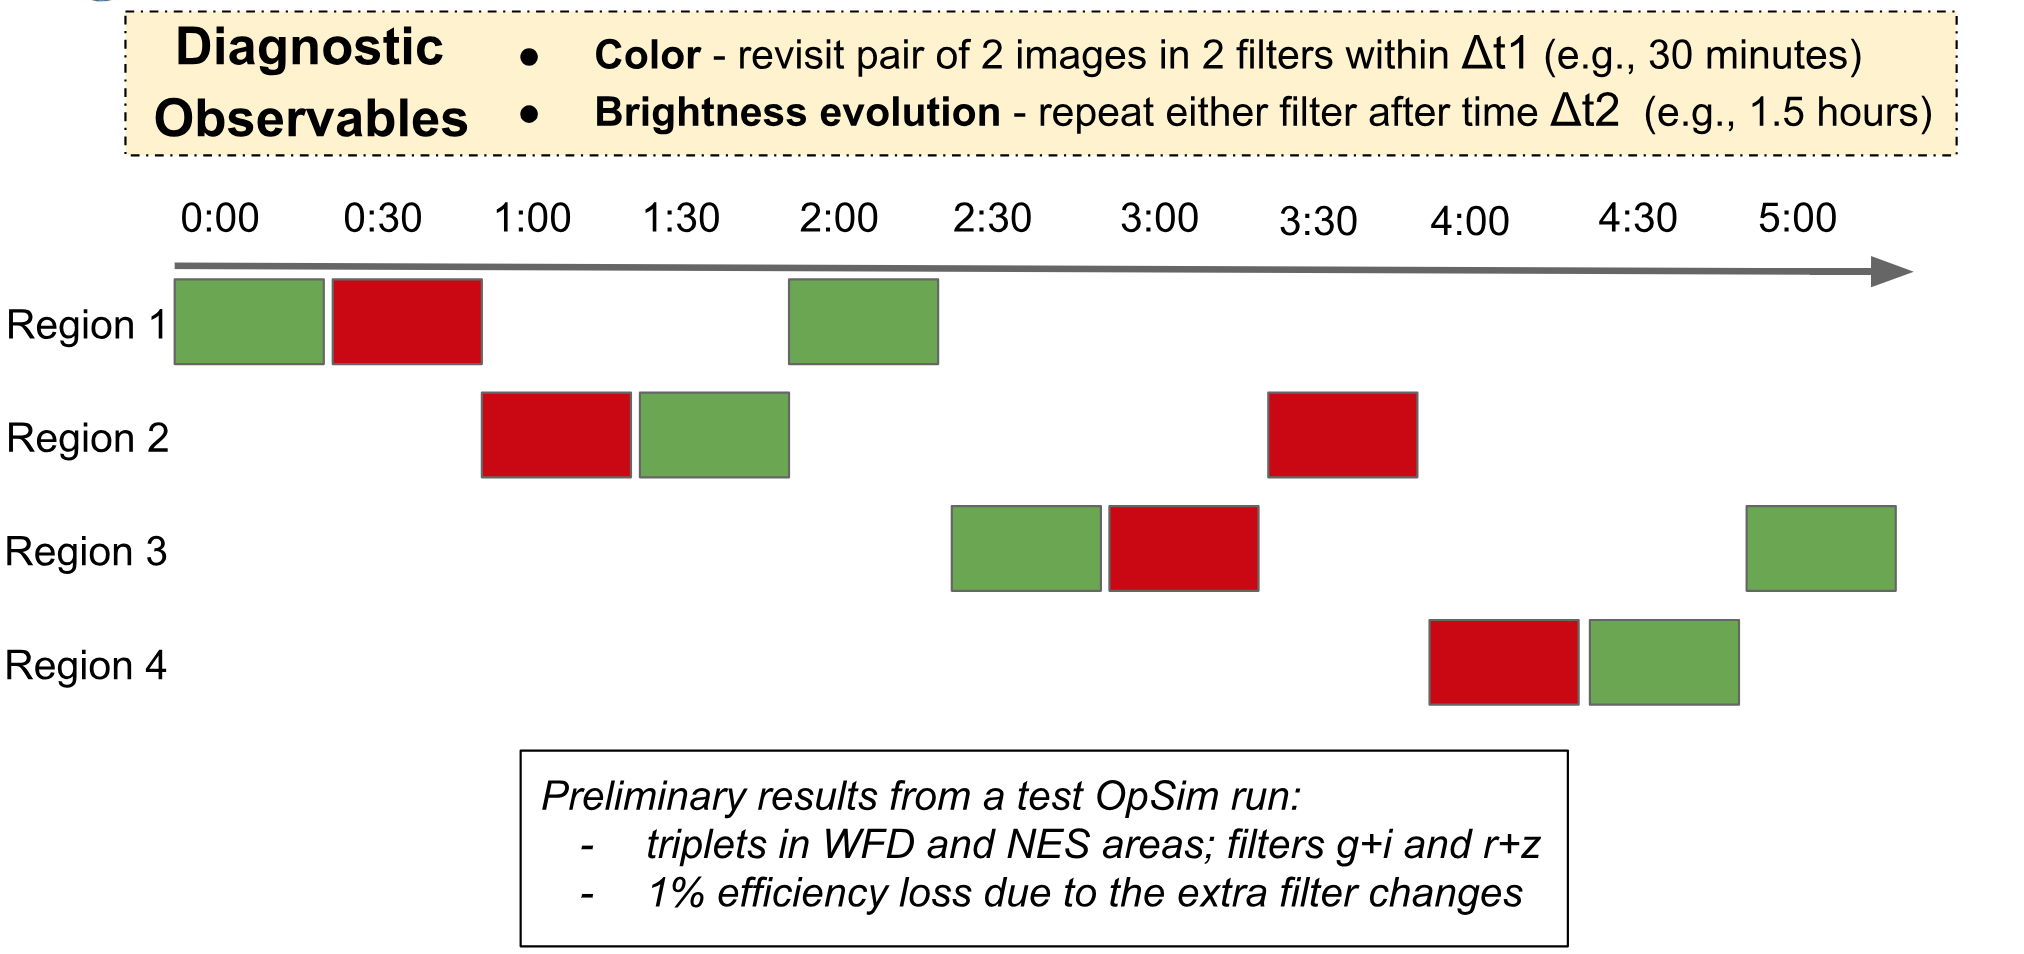
\includegraphics[width=0.9\textwidth]{figures/highLevelCadence.png}
\caption{Cadence example: two alternating filters cover regions of sky to obtain 3 observations per region, in 2 filters, with apprioriate time gaps to measure lightcurve color and shape.}
\end{figure}

\subsection{Footprint -- pointings, regions and/or constraints}
\begin{footnotesize}{\it Describe the specific pointings or general region (RA/Dec, Galactic longitude/latitude or Ecliptic longitude/latitude) for the observations. Please describe any additional requirements, especially if there are no specific constraints on the pointings (e.g. stellar density, galactic dust extinction).}
\end{footnotesize}

This proposed cadence does not make any additional constraints on the imaging area compared to WFD. The science goals might be reachable if the proposed cadence was implemented over a sub-region of the WFD survey area.  

\subsection{Image quality}
\begin{footnotesize}{\it Constraints on the image quality (seeing).}\end{footnotesize}

This proposed cadence does not make any additional constraints on the image quality compared to WFD. 

\subsection{Individual image depth and/or sky brightness}
\begin{footnotesize}{\it Constraints on the sky brightness in each image and/or individual image depth for point sources. Please differentiate between motivation for a desired sky brightness or individual image depth (as calculated for point sources). Please provide sky brightness or image depth constraints per filter.}
\end{footnotesize}

Should be the same as WFD standars

\subsection{Co-added image depth and/or total number of visits}
\begin{footnotesize}{\it  Constraints on the total co-added depth and/or total number of visits. Please differentiate between motivations for a given co-added depth and total number of visits. Please provide desired co-added depth and/or total number of visits per filter, if relevant.}
\end{footnotesize}

Should be the same as WFD standards.

\subsection{Number of visits within a night}
\begin{footnotesize}{\it Constraints on the number of exposures (or visits) in a night, especially if considering sequences of visits.  }
\end{footnotesize}

The proposed candence requires at least 3 visits per night.

\subsection{Distribution of visits over time}
\begin{footnotesize}{\it Constraints on the timing of visits --- within a night, between nights, between seasons or between years (which could be relevant for rolling cadence choices in the WideFastDeep. Please describe optimum visit timing as well as acceptable limits on visit timing, and options in case of missed visits (due to weather, etc.). If this timing should include particular sequences of filters, please describe.}
\end{footnotesize}

3 obs in 2 filters, 2 in different filters separated by <45 min, 1 in one of those filters separated by (?)>1.5 hour.

and the next visit - do we need to come back in the same filter? 

extragalactic fields that are being included in rolling cadence

and maybe some GP fields (microlensing events on short timescales; binary stars and BH, not exoplanets)

\subsection{Filter choice}
\begin{footnotesize}
{\it Please describe any filter constraints not included above.}
\end{footnotesize}

Filters should be pair with a gap in the sequence: g-i or r-z.                                                       
\subsection{Exposure constraints}
\begin{footnotesize}
{\it Describe any constraints on the minimum or maximum exposure time per visit required (or alternatively, saturation limits). Please comment on any constraints on the number of exposures in a visit.}
\end{footnotesize}

This proposed cadence uses the baseline exposure times of $2\times15$ seconds or $1\times30$ seconds.

\subsection{Other constraints}
\begin{footnotesize}
{\it Any other constraints.}
\end{footnotesize}

\subsection{Estimated time requirement}
\begin{footnotesize}
{\it Approximate total time requested for these observations, using the guidelines available at \url{https://github.com/lsst-pst/survey_strategy_wp}.}
\end{footnotesize}

Since our proposed cadence is a modification of the WFD strategy -- a shuffling of the visits, not adding visits -- it does not request any additional time.

\vspace{.3in}

\begin{table}[ht]
    \centering
    \begin{tabular}{l|l|l|l}
        \toprule
        Properties & Importance \hspace{.3in} \\
        \midrule
        Image quality &     \\
        Sky brightness &  \\
        Individual image depth &   \\
        Co-added image depth &   \\
        Number of exposures in a visit   &   \\
        Number of visits (in a night)  &   \\ 
        Total number of visits &   \\
        Time between visits (in a night) &  \\
        Time between visits (between nights)  &   \\
        Long-term gaps between visits & \\
        Other (please add other constraints as needed) & \\
        \bottomrule
    \end{tabular}
    \caption{{\bf Constraint Rankings:} Summary of the relative importance of various survey strategy constraints. Please rank the importance of each of these considerations, from 1=very important, 2=somewhat important, 3=not important. If a given constraint depends on other parameters in the table, but these other parameters are not important in themselves, please only mark the final constraint as important. For example, individual image depth depends on image quality, sky brightness, and number of exposures in a visit; if your science depends on the individual image depth but not directly on the other parameters, individual image depth would be `1' and the other parameters could be marked as `3', giving us the most flexibility when determining the composition of a visit, for example.}
        \label{tab:obs_constraints}
\end{table}

\subsection{Technical trades}
\begin{footnotesize}
{\it To aid in attempts to combine this proposed survey modification with others, please address the following questions:
\begin{enumerate}
    \item What is the effect of a trade-off between your requested survey footprint (area) and requested co-added depth or number of visits?
    \item If not requesting a specific timing of visits, what is the effect of a trade-off between the uniformity of observations and the frequency of observations in time? e.g. a `rolling cadence' increases the frequency of visits during a short time period at the cost of fewer visits the rest of the time, making the overall sampling less uniform.
    \item What is the effect of a trade-off on the exposure time and number of visits (e.g. increasing the individual image depth but decreasing the overall number of visits)?
    \item What is the effect of a trade-off between uniformity in number of visits and co-added depth? Is there any benefit to real-time exposure time optimization to obtain nearly constant single-visit limiting depth?
    \item Are there any other potential trade-offs to consider when attempting to balance this proposal with others which may have similar but slightly different requests?
\end{enumerate}}
\end{footnotesize}


\clearpage
%%%%%%%%%%%%%%%%%%%%%%%%%%%%%%%%%%%%%%%%%%%%%%%%%%%
\section{Performance Evaluation}
\begin{footnotesize}
{\it Please describe how to evaluate the performance of a given survey in achieving your desired science goals, ideally as a heuristic tied directly to the observing strategy (e.g. number of visits obtained within a window of time with a specified set of filters) with a clear link to the resulting effect on science. More complex metrics which more directly evaluate science output (e.g. number of eclipsing binaries successfully identified as a result of a given survey) are also encouraged, preferably as a secondary metric. If possible, provide threshold values for these metrics at which point your proposed science would be unsuccessful and where it reaches an ideal goal, or explain why this is not possible to quantify. While not necessary, if you have already transformed this into a MAF metric, please add a link to the code (or a PR to \href{https://github.com/lsst-nonproject/sims_maf_contrib}{sims\_maf\_contrib}) in addition to the text description. (Limit: 2 pages).}
\end{footnotesize}

\subsection{Diagnostic Metric}

Based on our evaluation of the light curves of fast transients, and the fast features of longer duration transients, we create a {\it diagnostic} metric that checks for the frequency with which the LSST observing simulation executes our desired filter-revisit cadence.

\subsection{The Other Kind of Metric}

The metric is the fraction of events for which the color and risetime is constrained (within some accuracy). Different science cases may have different input lightcurves and different gap requirements


\subsection{Create OpSim}

Tiago is setting up an {\tt OpSim} run that will do $f_1$ then 30 min later come back and do $f_2$, and then 60 min later come back and do $f_1$ or $f_2$, where $f_1$ and $f_2$ are $g$ and $i$, or $r$ and $z$. Non-adjacent filters are used to get a better leverage on the SED color.

\vspace{.6in}

\clearpage
%%%%%%%%%%%%%%%%%%%%%%%%%%%%%%%%%%%%%%%%%%%%%%%%%%%
\section{Special Data Processing}
\begin{footnotesize}
{\it Describe any data processing requirements beyond the standard LSST Data Management pipelines and how these will be achieved.}
\end{footnotesize}

The science goals that motivate the proposed cadence in this white paper will not require any data processing outside of the planned Prompt and Data Release pipelines and their data products. 

%%%%%%%%%%%%%%%%%%%%%%%%%%%%%%%%%%%%%%%%%%%%%%%%%%%
\section{References}
\bibliographystyle{aasjournal}

\bibliography{main}

\end{document}
